\documentclass[12pt]{article}

%%%%%%%%%%%%%%%%%
% the packages
\usepackage[utf8]{inputenc}
\usepackage[a4paper,margin=1in]{geometry}
\usepackage{graphicx,caption,subcaption}
\graphicspath{{./figures}}
\usepackage{color,hyperref}
\hypersetup{colorlinks=true,urlcolor=blue,citecolor=blue,linkcolor=blue}
\usepackage{enumitem}

\usepackage{multicol,longtable,multirow,booktabs,array}
\usepackage[authoryear]{natbib}
\bibliographystyle{plainnat}

\usepackage{mathaddons}

\newcommand{\sr}[1]{\textcolor{red}{#1}}


%%%%%%%%%%%%%%%%%%%%%%%%%
\title{Notes on High Dimension Probability}
\author{Subhrajyoty Roy}
\date{\today}


\begin{document}
\allowdisplaybreaks
\maketitle

\begin{abstract}
    This contains the lecture notes of the course on \textit{High Dimensional Probability} by Roman Vershynin. The course is available for free at online~\url{https://www.math.uci.edu/~rvershyn/teaching/hdp/hdp.html}.
\end{abstract}

\tableofcontents


\section{Introduction to High Dimensional Ideas}

\textbf{Big data} can come in one of two different ways.
\begin{enumerate}
    \item \# observations is big, this is usually easy, as classical statistical theory tells us how to deal with large number of samples. These are often better.
    \item \# dimensions is big. This is usually hard.
\end{enumerate}

Empirical observation: it is exponentially harder to deal with larger \# of dimensions rather than larger \# of observations. To illustrate this, let's consider an example problem.

\begin{example}
    Let's say we want to numerically compute the integral
    \begin{equation*}
        \int_0^1 \cdots \int_0^1 f(x_1, \ldots, x_d) dx_1 \ldots dx_d
    \end{equation*}
    The usual way is to perform a numerical integration approach, based on Riemann sums. For $d = 1$, we can subdivide the interval $[0, 1]$ into grids of width (or resolution) $\epsilon$, so there are $1/\epsilon$-grids. Then, we have the Riemann sum as
    \begin{equation*}
        \int_{[0, 1]} f(x)dx \approx \dfrac{1}{n}\sum_{i=1}^n f(x_i), \ n = (1/\epsilon).
    \end{equation*}
    \noindent Note that, this will ensure that the bias is of order $O(\epsilon)$, assuming $f$ is bounded. To see this,
    \begin{align*}
        \left\vert \int_{[0, 1]} f(x)dx - \dfrac{1}{n}\sum_{i=1}^n f(x_i) \right\vert
         & \leq \dfrac{1}{n}\sum_{i=1}^{n} \left\vert \int_{[(i-1)/n, i/n]} f(x)dx - f(x_i) \right\vert \\
         & = \dfrac{1}{n}\sum_{i=1}^{n} \left\vert f(t_i) - f(x_i) \right\vert                          \\
         & = O(1/n) = O(\epsilon)
    \end{align*}
    \noindent where $t_i$ is a tag obtained by using Integral Mean Value Theorem on $f$, for the interval $[(i-1)/n, i/n]$.

    In general, for $d$-dimensional hypercube $[0, 1]^d$, we require $n = O(1/\epsilon^d)$ many points to achieve an error bound of $O(\epsilon)$.
\end{example}

Therefore, we need the number of points to be exponential in dimension to achieve the same level of accuracy. This is also called \textbf{the curse of dimensionality}.

However, there is a better way to solve this problem, by using Monte Carlo method, which uses probabily to achieve good result for this. Instead of choosing the points on the grid, choose uniformly at random. Pick $N$ points:

\begin{equation*}
    S_N = \dfrac{1}{N}\sum_{i=1}^N f(x_i), \ x_i \sim \text{Uniform}([0, 1]^d)
\end{equation*}

Note that, $\E(S_N) = \E(f(X)) = \int_{[0, 1]^d} f(x)dx$. The average $L^2$ error is given by
\begin{align*}
    \E\left[\left(\frac{1}{N} \sum_{i=1}^N f(x_i) - \int_{[0,1]^d} f(x) dx\right)^2 \right]
     & = \var\left( \frac{1}{N} \sum_{i=1}^N f(x_i) \right) \\
     & = \dfrac{\var(f(X))}{N} \leq C/N
\end{align*}
\noindent since $f(x)$ is bounded. Therefore, the RMSE = $O(\frac{1}{\sqrt{N}})$, independent of the dimension $d$.

\begin{note}
    Thinking in terms of probability might help to overcome in high-dimensional inference problems.
\end{note}


\subsection{Convexity}

Usually in high-dimensional (HD) problems, convexity helps a lot.

\begin{definitionbox}
    A set $T \subset \R^n$ is convex if $\forall x,y \in T$, the segment $[x,y] \in T$.
\end{definitionbox}

Let us consider a few examples as follows:

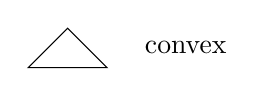
\begin{tikzpicture}[scale=0.5]
    \draw (0,0) -- (1,1) -- (2,0) -- cycle;
    \node at (4,0.5) {convex};
\end{tikzpicture}


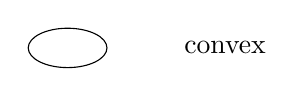
\begin{tikzpicture}[scale=0.5]
    \draw (3,0) ellipse (1cm and 0.5cm);
    \node at (7, 0) {convex};
\end{tikzpicture}


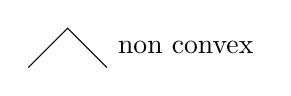
\begin{tikzpicture}[scale=0.5]
    \draw (6,0) -- (7,1) -- (8,0);
    \node at (10,0.5) {non convex};
\end{tikzpicture}


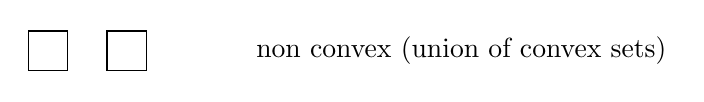
\begin{tikzpicture}[scale=0.5]
    \draw (9,0) rectangle (10,1);
    \draw (11,0) rectangle (12,1);
    \node at (20,0.5) {non convex (union of convex sets)};
\end{tikzpicture}

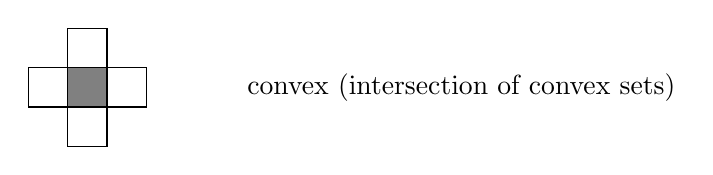
\begin{tikzpicture}[scale=0.5]
    \draw (5,0) rectangle (8,1);
    \draw (6,-1) rectangle (7,2);
    \draw[fill = gray] (6,0) rectangle (7,1);
    \node at (16,0.5) {convex (intersection of convex sets)};
\end{tikzpicture}

This means union of convex sets may not be convex, but intersection of convex sets is convex. Thus, starting with a set $T$, we can consider the intersection of all such convex sets that are superset of $T$.

\begin{definitionbox}
    The convex hull $\text{conv}(T)$ of a set $T \subset \R^n$ is the smallest convex set that contains $T$.
\end{definitionbox}

\begin{theorembox}
    $\forall z \in \text{conv}(T)$, we have a decomposition, $z = \sum_{i=1}^m \lambda_i z_i$, where, $\lambda_i \geq 0$, $\sum_{i=1}^m \lambda_i = 1$, and each $z_i \in T$. Note that, the above combination or representation may not be unique or parsimonious.
\end{theorembox}

\begin{theorembox}[Caratheodory Theorem]
    $\forall z \in \text{conv}(T)$, $\exists$ a representation (convex combination) of $\leq (n+1)$ points in $T$, where, $T \subset \R^n$.
\end{theorembox}

Note that, the choice of basis in the representation obtained by the Caratheodory Theorem may depend on the choice of $z$. Also, the number $(n+1)$ is unimprovable, there is a dimension dependence here. However, it turns out that if we allow to get $z$ back only approximately, we can use a similar trick like the Monte Carlo method to get a better representation, that may be dimension-independent. Additionally it says that we can choose the weights to be the same, and still get a good approximate solution.

\begin{theorembox}[Approximate Caratheodory Theorem]
    Let $T \subset \R^n$, and $\text{diam}(T) \leq 1$ (otherwise we can rescale). Then, $\forall z \in \text{conv}(T)$, $\forall k \in \N$, $\exists z_1, z_2, \ldots, z_k \in T$ (these points may be same) such that
    \begin{equation*}
        \left\Vert z - \frac{1}{k} \sum_{i=1}^k z_i\right\Vert_2 \leq \frac{1}{\sqrt{2k}}
    \end{equation*}
    This means, if we want error to be less than equal to $\epsilon$, the choose, $k = \frac{1}{2\epsilon^2}$ (which is dimension free).
\end{theorembox}

\begin{proof}
    \textbf{This proof is also called Empirical Method of Maurey}.

    Fix any $z \in \text{conv}(T)$, by Caratheory Theorem, we have, $z = \sum_{i=1}^m \lambda_i z_i$, $\lambda_i \geq 0$, $\sum_{i=1}^m \lambda_i = 1$, $z_i \in T$.

    Now, consider a random variable (r.v.) $Z$ that takes value $z_i$, with probability $\lambda_i$. Then, $\E(Z) = \sum_{i=1}^m \lambda_i z_i = x$. Let, $X_1, X_2, \dots X_k \equiv Z$ be iid copies of $Z$. Therefore, the $L^2$ error is
    \begin{align*}
        \E\left(\left\Vert z - \frac{1}{k} \sum_{i=1}^k X_i\right\Vert_2^2\right)
         & = \E\left\Vert \frac{1}{k} \sum_{i=1}^k (X_i - z)\right\Vert_2^2                                           \\
         & = \frac{1}{k^2} \sum_{i=1}^k \E\left\Vert X_i - \E(X_i)\right\Vert_2^2, \text{ since } z = \E(Z) = \E(X_i) \\
         & = \frac{1}{k} \E\left\Vert Z - \E(Z)\right\Vert_2^2, \text{ since } X_i \equiv Z                           \\
         & = \frac{1}{2k} \E\left\Vert Z - Z'\right\Vert_2^2, \text{ where } Z' \text{ is an independent copy of } Z  \\
         & \leq \frac{1}{2k}, \text{ as } \left\Vert Z-Z'\right\Vert_2^2 \leq \text{diam}(T) \leq 1
    \end{align*}

    \noindent So since, the expectation $\leq \frac{1}{2k} \Rightarrow \exists$ a realization of $X_i$'s such that $L^2$ error $\leq \frac{1}{2k}$. Therefore, $\left\Vert z - \frac{1}{k} \sum_{i=1}^k z_i\right\Vert_2^2 \leq \frac{1}{2k}$, where, $z_i$'s are the realizations of $X_i$, and hence each $z_i \in T$.
\end{proof}

\begin{exercisebox}
    Let $x_1, x_2, \dots x_n$ be an arbitrary set of unit vectors in $\R^n$. Prove that there exists $\epsilon_1, \epsilon_2, \dots, \epsilon_n$ with $\epsilon_i \in \{-1, +1\}$ such that $\Vert \sum_{i=1}^n \epsilon_i x_i\Vert_2 \leq \sqrt{n}$.

    To solve this, we use probabilistic methods. Note that, if $\epsilon_i$s are random variables, then the expected squared $L^2$ norm is
    \begin{equation*}
        \E\Vert \sum_{i=1}^n \epsilon_i x_i\Vert_2^2 = \sum_{i=1}^n \Vert x_i\Vert^2 \E(\epsilon_i^2) = n
    \end{equation*}
    \noindent since $x_i$ is unit vector and $\E(\epsilon_i^2) = \var(\epsilon_i) + \E^2(\epsilon_i) = 1$. This means, there exists a realization that has squared $L^2$ norm less than equal to $n$, i.e., the $L^2$ norm less than equal to $\sqrt{n}$.
\end{exercisebox}

\subsection{Applications of ACT}

There are multiple applications of ACT. One useful idea is in portfolio building, where the ingredients are ``stocks'', and their linear combination is basically a mutual fund. The problem is to create a new mutual fund with a given combination of stocks by mixing available mutual funds, (i.e., the fund of funds). The solution is to use ACT to obtain a fast randomized solution approximately.

\begin{note}
    Note that, ACT only provides the existence, and does not necessarily provide an algorithm to find that out. However, one simple algorithm could be to start with all the available mutual funds and then take any $k$ of them randomly and average their returns.
\end{note}

Another prominent application of ACT is in covering numbers. This is what we will explore now.

\begin{definitionbox}
    The \textbf{Covering Number} of a set $T \subset \mathbb{R}^n$ at scale $\epsilon > 0$ is the smallest \# of Euclidean balls of radius $\epsilon$ needed to cover $T$. It is denoted by $N(T,\epsilon)$.
\end{definitionbox}

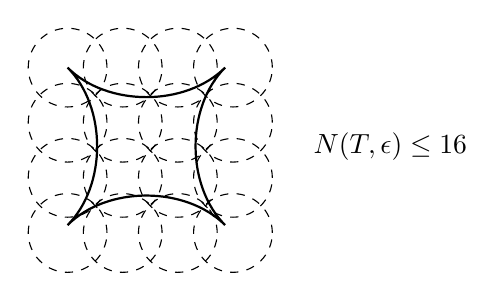
\begin{tikzpicture}
    % Draw the concave shape with four corners
    \draw[thick] (0,0) .. controls (0.5,-0.5) and (1.5,-0.5) .. (2,0)
    .. controls (1.5,-0.5) and (1.5,-1.5) .. (2,-2)
    .. controls (1.5,-1.5) and (0.5,-1.5) .. (0,-2)
    .. controls (0.5,-1.5) and (0.5,-0.5) .. (0,0);

    % Draw unit circles covering the shape
    \foreach \x in {0, 0.7, 1.4, 2.1} {
            \foreach \y in {0, -0.7, -1.4, -2.1} {
                    \draw[dashed, fill=none] (\x,\y) circle (0.5);
                }
        }
    \node[right] at (3,-1) {$N(T,\epsilon) \leq 16$};
\end{tikzpicture}

\begin{lemmabox}
    Let $B$ be the unit Euclidean ball, then we have $N(B, \frac{1}{2}) \geq 2^d$, i.e., the covering number is exponential in dimension.
\end{lemmabox}

\begin{proof}
    Assume $B$ can be covered by $N$ copies of $(\frac{1}{2}B)$ ball. Then clearly,
    \begin{align*}
                 & Vol(B) \leq N \cdot Vol\left(\frac{1}{2}B\right), \text{ since RHS might have some overlaps.} \\
        \implies & Vol(B) \leq N 2^{-d} Vol(B)                                                                   \\
        \implies & N \geq 2^d
    \end{align*}
\end{proof}

This is an unsurprising result. However, what is surprising is that the covering number for a polytope (i.e., a higher dimensional analogue of polygon), is independent of the dimension but dependent only on the number of vertices. Also, it is polynomial in the number of vertices.

\begin{lemmabox}
    Let $P$ be a polytope in $\R^d$ with $m$ vertices and $\text{diam}(P) \leq 1$. Then, $N(P, \epsilon) \leq m^{1/2\epsilon^2}$.
\end{lemmabox}
\begin{proof}
    If we consider, $P$ to be nonconvex, then $conv(P)$ is a polytope with $\leq m$ vertices. This can only weaken the bound. Therefore, it is enough to show it for the cases when $P$ is convex.

    Let $T$ be the set of vertices of $P$. Clearly, $P \subseteq conv(T)$. Note that ACT implies that $\forall z \in P$, is within distance $\frac{1}{\sqrt{2k}}$ from some point in the set
    \begin{equation*}
        \mathcal{N} := \left\{\frac{1}{k} \sum_{i=1}^k z_i : z_i \in T \right\}.
    \end{equation*}
    \noindent This means, $\forall x \in P$, is covered by a ball of radius $\frac{1}{\sqrt{2k}}$ and center $\in \mathcal{N}$. This means, the covering number
    \begin{equation*}
        N(P, 1/\sqrt{2k}) \leq \vert \mathcal{N}\vert \leq m^k,
    \end{equation*}
    \noindent since to choose an element of $\mathcal{N}$, we pick any $k$ vertices from $m$ vertices which is $\binom{m}{k} = O(m^k)$. Choosing $\epsilon = 1/\sqrt{2k}$ now completes the proof.
\end{proof}

To make use of these results, usually, it helps by considering the intuition that, a small covering \# $\Rightarrow$ small volume, $\Rightarrow$ easier to apply union-type bounds. As a result, since the covering number of a polytope is small, we expect the volume of the polytope also be to small compared to the Euclidean ball.

\begin{theorembox}[Carl-Pajor, 88]
    Let $B$ be the unit Euclidean ball, and $P \subset B$ be any polytope with $m$ vertices in $\R^n$. Then,
    \begin{equation*}
        \dfrac{Vol(P)}{Vol(B)} \leq \left( 4\dfrac{\sqrt{\log m}}{\sqrt{n}} \right)^n
    \end{equation*}
\end{theorembox}
\noindent What the Carl-Pajor theorem tells us is that the volume of the polytope is extremely small, unless the number of vertices $m$ is exponential in $n$.

\begin{proof}
    Let us consider $\epsilon B$-balls and cover $P$ with these balls. By definition of covering number, we have
    \begin{align*}
                 & Vol(P) \leq N(P,\epsilon) Vol(\epsilon B)                                   \\
        \implies & Vol(P) \leq N(P, \epsilon) \epsilon^n Vol(B)                                \\
        \implies & Vol(P)/Vol(B) \leq \epsilon N(P, \epsilon) \leq \epsilon^n m^{2/\epsilon^2}
    \end{align*}
    \noindent Here, we use the previous Lemma, but with the understanding that since $B$ is a unit Euclidean ball, its diameter is $2$. Now, note that the above inequality is true for every $\epsilon > 0$. Therefore,
    \begin{equation*}
        \frac{Vol(P)}{Vol(B)} \leq \inf_{\epsilon > 0} \epsilon^n \cdot m^{\frac{1}{2\epsilon^2}}.
    \end{equation*}
    \noindent Let $\ell(\epsilon) = \epsilon^n m^{\frac{1}{2\epsilon^2}} \Rightarrow \log \ell(\epsilon) = n \log \epsilon + \frac{1}{2\epsilon^2} \log m$. Now setting its derivative equal to $0$, we get $\frac{\partial \log l}{\partial \epsilon} = 0 = \frac{n}{\epsilon} - \frac{1}{\epsilon^3} \log m \Rightarrow \epsilon = \sqrt{\frac{4 \log m}{n}}$. Putting this value of $\epsilon$ based into the expression, we get
    \begin{align*}
        \inf_{\epsilon > 0} \ell(\epsilon)
         & = \exp\left[ n \log\left( \dfrac{\sqrt{4\log m}}{\sqrt{n}} \right) + \dfrac{2\log m}{4\log m} n \right] \\
         & = \exp\left[ \log\left( \dfrac{\sqrt{4\log m}}{\sqrt{n}} \right)^n e^{n/2} \right]                      \\
         & = \left( \dfrac{\sqrt{4e \log m}}{\sqrt{n}} \right)^n
        \leq \left( 4\dfrac{\sqrt{\log m}}{\sqrt{n}} \right)^n, \text{ since } e \leq 4.
    \end{align*}
\end{proof}

A few remarks we want to make here.
\begin{itemize}
    \item Carl-Pajor proved a slightly better result, with $\log(m/n)$ rate, which is optimal.
    \item The optimal bound is attained at a random polytope. (Dafnis et al., 2003, 2009)
    \item Let $\delta = 4\sqrt{\frac{\log m}{n}}$, then note that, $Vol(\delta B) = \delta^n \cdot Vol(B)$, and correspondingly, $\Rightarrow \frac{Vol(\delta B)}{Vol(B)} = \delta^n \geq \frac{Vol(P)}{Vol(B)}$. As a result, we have $Vol(\delta B) \geq Vol(P)$. This means, a small ball around origin has at least the same volume as the polytope.
\end{itemize}

This means, the low-dimensional picture that we usually think is wrong.

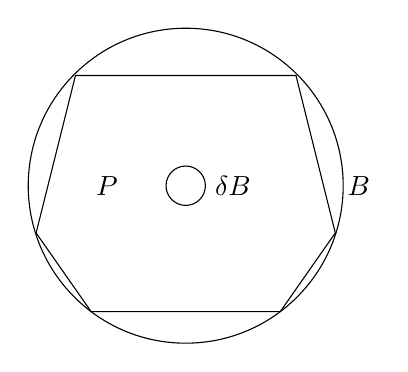
\begin{tikzpicture}
    \draw (0,0) circle (2cm);
    \draw (0,0) circle (0.25cm);
    \draw (-1.9,-0.6) -- (-1.4,1.4) -- (1.4,1.4) -- (1.9,-0.6) -- (1.2, -1.6) -- (-1.2, -1.6) -- cycle;
    \node at (-1,0) {$P$};
    \node at (0.6,0) {$\delta B$};
    \node at (2.2,0) {$B$};
\end{tikzpicture}

\noindent For correct intuition in high dimension, we can consider the hyperbolic correction by ``V. Milman''.

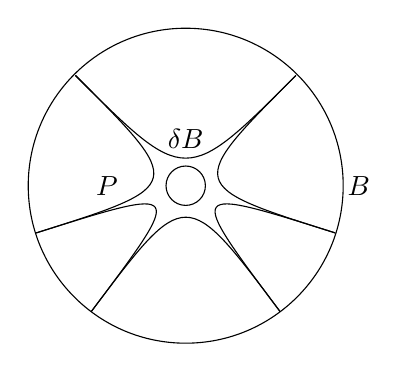
\begin{tikzpicture}
    \draw (0,0) circle (2cm);
    \draw (0,0) circle (0.25cm);
    \draw (-1.9, -0.6) .. controls (0, 0) .. (-1.4, 1.4);
    \draw (-1.4, 1.4) .. controls (0, 0) .. (1.4, 1.4);
    \draw (1.4, 1.4) .. controls (0, 0) .. (1.9, -0.6);
    \draw (1.2, -1.6) .. controls (0, 0) .. (1.9, -0.6);
    \draw (1.2, -1.6) .. controls (0, 0) .. (-1.2, -1.6);
    \draw (-1.9, -0.6) .. controls (0, 0) .. (-1.2, -1.6);
    \node at (-1,0) {$P$};
    \node at (0,0.6) {$\delta B$};
    \node at (2.2,0) {$B$};
\end{tikzpicture}

\noindent The part $\delta B$ is called the ``core'' of the polytope. Note that, the polytope is convex, but it does not look convex. This is because, for high dimensional inference, we cannot completely visualize all the information. So here, we drop the convexity (because we can work with it algebraically), and instead work with the volume-based ideas (because probabilities map to volume in terms of measures).


\pagebreak
\section{Concentration Inequalities}

We know by law of large numbers that i.i.d. sum of a random variable $\bb{X}$ converges to $\E(X)$. The central limit theorem also tells that the rate of this convergence is $1/\sqrt{n}$. Since the central limit theorem and law of large numbers are very universal in nature, one might want to know to what extent these kinds of concentration holds. The fundamental aim of concentration inequalities is to demonstrate that a random variable (or i.i.d. sum of it) satisfies $X \approx \E(X)$ with high probability (exponentially close to $1$).

For example, in case of normal distribution, $X \sim N(\mu, \sigma^2)$, we know that
\begin{equation*}
    \prob(\vert X - \mu\vert > 3\sigma) = 0.9973.
\end{equation*}

For general distribution, we have
\begin{align*}
    \prob(X \geq t)                 & \leq \dfrac{\E(X)}{t}, \ \forall t > 0, \ \text{(because of Markov's inequality)}       \\
    \prob(\vert X - \E(X)\vert > t) & \leq \dfrac{\sigma^2}{t^2}, \ \forall t > 0, \ \text{because of Chebyshev's inequality}
\end{align*}

However, for Gaussian distribution, the concentration around the mean is much faster. To see this, consider the following Lemma.

\begin{theorembox}
    Suppose $g \sim N(0, 1)$, then
    \begin{equation*}
        \prob(g > t) \leq \frac{1}{\sqrt{2\pi}} \frac{e^{-t^2/2}}{t},
    \end{equation*}
    \noindent i.e., the tail probability decays exponentially fast in $t$.
\end{theorembox}
\begin{proof}
    \begin{align*}
        \prob(g > t) & = \int_{t}^{\infty} \frac{1}{\sqrt{2\pi}} e^{-x^2/2}dx                                               \\
                     & = \int_{0}^{\infty} \frac{1}{\sqrt{2\pi}} e^{-(t+y)^2/2} dy, \text{ using substitution } x = y + t   \\
                     & = \int_{0}^{\infty} \frac{1}{\sqrt{2\pi}} e^{-t^2/2} e^{-ty} e^{-y^2/2} dy                           \\
                     & \leq \int_{0}^{\infty} \frac{1}{\sqrt{2\pi}} e^{-t^2/2} e^{-ty} dy, \text{ since } e^{-y^2/2} \leq 1 \\
                     & = \frac{1}{\sqrt{2\pi}} e^{-t^2/2} \int_{0}^{\infty} e^{-ty} dy                                      \\
                     & = \dfrac{1}{\sqrt{2\pi} t} e^{-t^2/2}
    \end{align*}
\end{proof}

By symmetry, then we have for general $X \sim N(\mu, \sigma^2)$,
\begin{equation*}
    \prob(\vert X -\mu \vert > t\sigma) \leq \dfrac{1}{t}\sqrt{\dfrac{2}{\pi}} e^{-t^2/2} \leq e^{-t^2/2}, \text{ when } t \geq 1.
\end{equation*}

Therefore, the normal distribution has exponential tails.  Also, the central limit theorem (CLT) tells that
\begin{equation*}
    \sqrt{n} \left(\frac{\bar{X} - \mu}{\sigma}\right) \xrightarrow{d} Z \sim N(0,1),
\end{equation*}
\noindent so may be the tail probabilities are also close and exponential. But this does not work as the error from the CLT itself is of order $O(1/\sqrt{n})$, which is due to Berry-Esseen bound. So, the tail of $\sqrt{n} \left(\frac{\bar{X} - \mu}{\sigma}\right)$ does exponentially decay in general like Gaussian, at least by this route.

\begin{theorembox}[Berry Essen Bound]
    Let $X_i$ be i.i.d. random variables with mean $0$ and variance $1$, and finite third order moment. Then,
    \begin{equation*}
        \left\vert \prob\left( \dfrac{1}{\sqrt{N}}\sum_{i=1}^N X_i \geq t \right) - \prob(Z \geq t) \right\vert \leq \dfrac{\E(\vert X_1\vert^3}{\sqrt{N}} = O(1/\sqrt{N}),
    \end{equation*}
    \noindent where $Z \sim N(0, 1)$.
\end{theorembox}

\noindent So we would like to sidestep this CLT and try to control the tail of this normalized sum directly. This introduces the study of concentration inequalities.

\begin{exercisebox}
    Let $X$ be a standard normal random vector in $\R^n$ where $n \geq C_1$ (large constant). What are the values of $\E\Vert X\Vert_2^2$ and $\var(\Vert X\Vert_2^2)$?

    To obtain this, let $X_1, X_2, \dots X_n$ be the coordinates of the vector, note that
    \begin{align*}
        \E\Vert X\Vert_2^2     & = \E(X_1^2 + X_2^2 + \dots + X_n^2) = n \E(X_1^2) = n                                       \\
        \var(\Vert X\Vert_2^2) & = \var(X_1^2 + \dots + X_n^2) = n\var(X_1^2) = n\left[ \E(X_1^4) - \E^2(X_1^2) \right] = 2n
    \end{align*}
\end{exercisebox}

\begin{exercisebox}[Continued]
    Show that, $\vert \Vert X\Vert_2^2 - n\vert \leq C \sqrt{n}$ for some large $C$ with high probability (say $0.99$).

    To show this, we make use of Chebyshev's inequality. Note that,
    \begin{equation*}
        \prob(\vert \Vert X\Vert_2^2 - n\vert > t) = \prob(\vert \Vert X\Vert_2^2 - \E(\Vert X\Vert_2^2) \vert > t) \leq \dfrac{\var(\Vert X\Vert_2^2)}{t^2} = \dfrac{2n}{t^2}
    \end{equation*}
    \noindent Choosing $t = C\sqrt{n}$ for large $C$ yields, $\prob(\vert \Vert X\Vert_2^2 - n\vert > C\sqrt{n}) \leq 2/C$, which can be made smaller than $0.01$ by choosing large $C$.
\end{exercisebox}

\begin{exercisebox}[Continued]
    Deduce that this means, $\sqrt{n}/2 \leq \Vert X\Vert_2 \leq 2\sqrt{n}$ with high probability say $0.99$.

    Note that,
    \begin{equation*}
        \vert \Vert X\Vert_2 - \sqrt{n} \vert = \dfrac{\vert \Vert X\Vert_2^2 - n \vert}{\vert \Vert X\Vert_2 + \sqrt{n} \vert} = \dfrac{\leq C\sqrt{n}}{\geq \sqrt{n}} \leq C
    \end{equation*}
    \noindent with high probability. This says that for a random normal vector $X$, $\Vert X\Vert_2 = \sqrt{n} + o(1)$.
\end{exercisebox}

\begin{exercisebox}
    Let $X$ and $Y$ be two independent standard normal random vectors in $\R^n$ for some $n \geq C$. Find $\E\inner{X,Y}^2$ and $\var\inner{X,Y}^2$.

    Note that,
    \begin{align*}
        \E\inner{X,Y}^2
         & = \E\left( (\sum_{i=1}^n X_i Y_i)^2 \right)                                    \\
         & = \E\left[ \sum_{i=1}^n X_i^2 Y_i^2 + \sum_{i \neq j} X_iX_jY_iY_j \right] = n
    \end{align*}
    \noindent since $\E(X_i^2Y_i^2) = \E(X_i^2)\E(Y_i^2)$, by independence, and the second term is zero.

    Similarly,
    \begin{align*}
        \E\inner{X,Y}^4
         & = \E\left[ \left( \sum_{i=1}^n X_iY_i \right)^4 \right]                                                             \\
         & = \E\left[ \sum_{i=1}^n X_i^4 Y_i^4 + \sum_{i \neq j} X_i^2 Y_i^2 X_j^2 Y_j^2 \right], \text{ other terms are zero} \\
         & = n \times 3 \times 3 + n(n-1) \times 1 = n^2 + 8n
    \end{align*}
    \noindent Therefore, $\var\inner{X,Y}^2 = \E\inner{X,Y}^4 - \E^2\inner{X,Y}^2 = n^2 + 8n - n^2 = 8n$.
\end{exercisebox}

\begin{exercisebox}[(Continued)]
    Show that if the angle between those vectors is denoted by $\theta$, then $\vert \theta - \pi/2\vert = O(1/\sqrt{n})$ with large probability.

    We start by applying Chebyshev's inequality on $\inner{X,Y}^2$. Note that,
    \begin{equation*}
        \prob\left( \vert \inner{X,Y}^2 - n\vert \geq 3n \right) \leq \dfrac{\var\inner{X,Y}^2}{9n^2} = \dfrac{8}{9n} \rightarrow 0
    \end{equation*}
    \noindent Therefore, with sufficiently large probability, $\inner{X,Y}^2 \leq 4n$. This means,
    \begin{equation*}
        \cos^2(\theta) = \dfrac{\inner{X,Y}^2}{\norm{X}_2^2 \norm{Y}_2^2} = \dfrac{\leq 4n}{\geq (\sqrt{n} + o(1))^4} \leq \dfrac{C_2}{n}
    \end{equation*}
    \noindent i.e., $\vert \cos(\theta)\vert = O(1/\sqrt{n})$. Here we apply the result from previous exercise that $\norm{X}_2^2 = (\sqrt{n}+o(1))$. Therefore, $\vert \theta - \pi/2\vert = O(1/\sqrt{n}) \rightarrow 0$ as $n \rightarrow \infty$.
\end{exercisebox}

What this exercise shows is that in high dimensions, almost any pair of unit random vectors are orthogonal to each other.


\subsection{Inequalities}

\begin{definitionbox}
    A symmetric Bernoulli random variable is $X$ which takes values $+1$ and $(-1)$ with equal probabilities, i.e., $1/2$.
\end{definitionbox}

\begin{theorembox}[Hoeffding's inequality]
    Let $X_1, X_2, \dots X_N$ be symmetric Bernoulli random variables, then
    \begin{equation*}
        \prob\left(\frac{1}{\sqrt{n}} \sum_{i=1}^{n} X_i \geq t\right) \leq e^{-t^2/2}, \quad \forall t \geq 0,
    \end{equation*}
    \noindent i.e., the normalized sum exhibits Gaussian tail behaviour.
\end{theorembox}
\begin{proof}
    \textbf{This proof is also known as the MGF method.}

    Let $\lambda > 0$ be a parameter. Then
    \begin{align*}
        \prob\left( \frac{1}{\sqrt{n}} \sum_{i=1}^{n} X_i \geq t \right)
         & = \prob\left(e^{\lambda \sum_{i=1}^{n} X_i} \geq e^{\lambda t \sqrt{n}}\right)                                                   \\
         & \leq e^{-\lambda t \sqrt{n}} \E\left(e^{\lambda \sum_{i=1}^{n} X_i}\right), \text{ by Markov's inequality}                       \\
         & = e^{-\lambda t \sqrt{n}} \prod_{i=1}^{n} \mathbb{E}\left(e^{\lambda X_i}\right), \text{ since } X_i\text{s are i.i.d.}          \\
         & = e^{-\lambda t \sqrt{n}} \left(\frac{e^{\lambda} + e^{-\lambda}}{2}\right)^n                                                    \\
         & \leq e^{-\lambda t \sqrt{n}} e^{n\lambda^2/2}, \text{ since } \cosh(\lambda) = (e^\lambda + e^{-\lambda})/2 \leq e^{\lambda^2/2} \\
         & = \exp\left( -\lambda t \sqrt{n} + n\lambda^2/2 \right)
    \end{align*}
    \noindent Now, we optimize this final bound over the choice of $\lambda > 0$ to complete the proof.
\end{proof}

The general version of Hoeffding's inequality can work with any bounded random variables. For example,

\begin{theorembox}
    Let \( X_1, X_2, \dots, X_n \) be i.i.d. r.v. such that \( X_i \in [a_i, b_i] \) for all $i$. Then, \( S_n = \sum_{i=1}^{n} X_i \) satisfies
    \begin{equation*}
        \prob\left( S_n - \E(S_n) \geq t\right) \leq \exp\left(-\frac{2 t^2}{\sum_{i=1}^{n} (b_i - a_i)^2}\right)
    \end{equation*}
\end{theorembox}

Unfortunately, there is one problem with Hoeffding's inequality. It works only for bounded random variables, and does not take into account the variance component. Therefore, it will yield the same bound for a uniform random variable on $[a, b]$ and the random variable that takes probability $1/2$ on both the endpoints of $[a, b]$. But we expect the former to have a rapid decay.

Let us consider an empirical approximation. Let $X_1, X_2, \dots X_N \sim \text{Ber}(p)$, such that $p \to 0$ and $pN \to \mu$. Then,
\begin{equation*}
    \prob\left(S_n = \sum_{i=1}^{n} X_i \geq t\right) \rightarrow \text{Poisson}(\mu)
\end{equation*}
\noindent Consider Poisson tails,
\begin{align*}
    \prob\left(\sum_{i=1}^{n} X_i \geq t\right)
     & = e^{-\mu} \sum_{k \geq t} \frac{\mu^k}{k!} \quad \text{(Stirling's bounds: } k! \sim \sqrt{2 \pi k}\left(\frac{k}{e}\right)^k) \\
     & \sim e^{-\mu} \mu^t \left(\frac{e}{t}\right)^t \quad \text{(only dominating term is } t)                                        \\
     & = e^{-\mu} \left(\frac{\mu e}{t}\right)^t = O((C/t)^{-t})
\end{align*}
\noindent Hence, we expect a tail that is like $t^{-t}$, or $e^{-t\log(t)}$, instead of the lighter Gaussian tail $e^{-t^2/2}$. This is illustrated through Chernoff's inequality.

\begin{theorembox}[Chernoff's inequality]
    Let $X_i \sim \text{Ber}(p_i)$, and $S_N = \sum_{i=1}^N X_i$ has mean $\E(S_N) = \sum_{i=1}^N p_i = \mu$, and satisfies,
    \begin{equation*}
        \prob(S_N \geq t) \leq e^{-\mu}\left( \dfrac{e\mu}{t} \right)^t, \ \forall t \geq \mu
    \end{equation*}
\end{theorembox}

\begin{proof}
    Using the MGF method, we have $\prob\left(S_n \geq t\right) \leq e^{-\lambda t} \prod_{i=1}^{N} \mathbb{E}\left(e^{\lambda X_i}\right)$. Now note that,
    \begin{equation*}
        \E\left(e^{\lambda X_i}\right) = e^{\lambda}p_i + (1 - p_i) \leq 1 + \left(e^{\lambda} - 1\right)p_i \leq \exp\left(\left(e^{\lambda} - 1\right) p_i\right) \quad (\text{as } 1 + x \leq e^x)
    \end{equation*}
    \noindent Therefore, we have
    \begin{equation*}
        \prob(S_N \geq t) \leq e^{-\lambda t} \exp\left[ (e^\lambda - 1)\mu \right] = \exp\left[ -\lambda t + (e^\lambda - 1)\mu \right].
    \end{equation*}
    \noindent Similar to before, we now optimize over the choices of $\lambda > 0$. Differentiating with respect to $\lambda$ yields, $(-t + e^\lambda \mu) = 0$, i.e., $\lambda = \log(t/\mu)$. Since $t \geq \mu$, this optimal value of $\lambda \geq 0$. Putting $\lambda = \log(t/\mu)$ back into the expression, we get
    \begin{equation*}
        \exp\left( -t\log(t/\mu) + (t/\mu - 1)\mu \right) = \exp\left( -\mu + t - t\log(t) + t\log(\mu) \right) = e^{-\mu}\left( \dfrac{e\mu}{t} \right)^t,
    \end{equation*}
    \noindent as we wanted.
\end{proof}

Although the Chernoff bound predicts a heavier tail compared to the Gaussian tail (i.e., $O(e^{-t \log(t)}$ instead of $O(e^{-t^2})$), it makes sense only when $t >> \mu$. When $t \approx \mu$, i.e., for small deviations, we can get Gaussian approximations.
\begin{align*}
    \prob(S_n \geq (1+\delta)\mu)
     & \leq e^{-\lambda \mu} \left(\frac{e}{1+\delta}\right)^{(1+\delta)\mu}, \text{ say } \delta \leq 1 \\
     & = \exp\left[ \mu\left( \delta - (1+\delta)\log(1+\delta) \right) \right]
\end{align*}
\noindent By Taylor series, we have
\begin{align*}
    \log(1+\delta)                             & = \delta - \delta^2/2 + \delta^3/3 + \dots \geq \delta - \delta^2/2                                                     \\
    \delta - (1+\delta)\log(1+\delta)          & \leq \delta - (1+\delta)(\delta - \delta^2/2) = \delta - (\delta + \delta^2 - \delta^2/2 - \delta^3/3) \leq -\delta^2/6 \\
    \prob\left( S_n \geq (1+\delta)\mu \right) & \leq \exp\left( -\delta^2\mu/6 \right), \ \forall \delta \leq 1,
\end{align*}
\noindent Note that, this is like a Gaussian tail. Therefore, what Chernoff bound shows is that near the center, this sum of Bernoulli's behave like Gaussian (so CLT and other approximations work well) but in the tail region, it is fatter than the Gaussian.

\begin{center}
    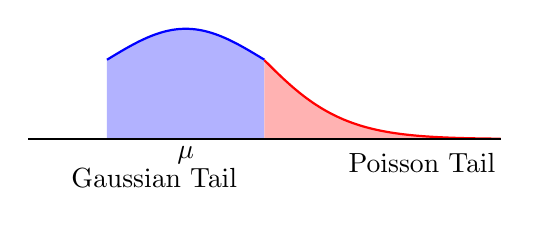
\begin{tikzpicture}
        % Plot and fill the first curve
        \fill[blue!30] (-1, 0) -- plot[domain=-1:1, smooth, variable=\x] ({\x}, {0.4 + exp(-\x*\x/2)}) -- (1, 0) -- cycle;
        \draw[domain=-1:1, smooth, variable=\x, blue, thick] plot ({\x}, {0.4 + exp(-\x*\x/2)});

        % Plot and fill the second curve, adjusting the domain and scaling for continuity
        \fill[red!30] (1, 0) -- plot[domain=1:4, smooth, variable=\x] ({\x}, {exp(-\x*ln(\x))}) -- (4, 0) -- cycle;
        \draw[domain=1:4, smooth, variable=\x, red, thick] plot ({\x}, {exp(-\x*ln(\x))});
        \draw (-2,0) -- (4,0);
        \node at (0, -0.2) {$\mu$};
        \node at (-0.4, -0.5) {Gaussian Tail};
        \node at (3, -0.3) {Poisson Tail};
    \end{tikzpicture}
\end{center}



\subsection{Applications}

\subsubsection{Mean estimation}

We start with an application of Hoeffding's inequality. Consider an i.i.d. sample \( X_1, X_2, \dots, X_n \) from $(\mu, \sigma^2)$, i.e., $\E(X_i) = \mu$ and $\var(X_i) = \sigma^2$. We want to estimate these parameters. The classical estimator of the population mean is the sample mean, i.e., $\widehat{\mu} = \dfrac{1}{n}\sum_{i=1}^n X_i$, and it turns out that $\E(\hat{\mu}) = \mu$ and hence it is unbiased, and also $\var(\hat{\mu}) = \sigma^2/n$. One can show that this is UMVUE, hence this rate of variance is optimal.

The usual confidence intervals in this case looks like $\left( \widehat{\mu} - t\sigma/\sqrt{n}, \widehat{\mu}+t\sigma/\sqrt{n} \right)$, for some $t$. However, this may not be very sharp or the best confidence interval. Because, we only get
\begin{equation*}
    \prob(\vert \hat{\mu} - \mu\vert \geq t\sigma/\sqrt{n}) \leq \dfrac{\sigma^2/n}{(t\sigma/\sqrt{n})^2} = \dfrac{1}{t^2},
\end{equation*}
\noindent by usage of Chebyshev's inequality. This is not a very sharp bound.

\textbf{Can we get sharper exponentially close to 1 confidence for general distributions? Surprisingly YES! (Note that we only assume \( \mathbb{E}|X|^2 < \infty \), not higher order moments)}.

This trick is called \textbf{Median of means} estimator. Assume $n = mK$. Partition the sample into $K$ blocks of size $m$, denoted as $B_1, B_2, \dots B_K$. Let, $\hat{\mu}_j = \dfrac{1}{m}\sum_{i \in B_j} X_i$. Define, $\tilde{\mu}$ to be the median of these blockwise means, i.e., median of $\hat{\mu}_1, \dots \hat{\mu}_K$.

The confidence interval is given in the same way as before, $\left( \tilde{\mu} - t\sigma/\sqrt{n}, \tilde{\mu}+t\sigma/\sqrt{n} \right)$, for some $t$. Note that, the error for each $\hat{\mu}_j$ is,
\begin{equation*}
    \prob\left(\hat{\mu}_j \geq \mu + \frac{t \sigma}{\sqrt{n}}\right) \leq \frac{\sigma^2/m}{(t \sigma/\sqrt{n})^2} = \frac{n/m}{t^2} = \frac{K}{t^2}
\end{equation*}
\noindent We can choose $K$ as per our convenience. Let us choose $K = t^2/4$. In this case,
\begin{equation*}
    \prob\left(\hat{\mu}_j \geq \mu + \frac{t \sigma}{\sqrt{n}}\right) \leq \frac{1}{4}.
\end{equation*}
\noindent Now, by definition of median, we have
\begin{equation*}
    \prob\left(\hat{\mu} > \mu + \frac{t \sigma}{\sqrt{n}}\right) \leq \prob\left(\text{at least } \frac{K}{2} \text{ of } \hat{\mu}_j \text{ are } \geq \frac{t \sigma}{\sqrt{n}}\right)
\end{equation*}
\noindent Note that, $Y_j = \bb{1}(\hat{\mu}_j \geq t\sigma/\sqrt{n}) \sim \text{Ber}(p)$, where $p \leq 1/4$. Let, $S_K = \frac{1}{K}\sum_{i=1}^K Y_j$. Then, $\E(S_K) = Kp \leq K/4$ and $\var(S_K) = Kp(1-p) \leq 3K/16$. Hence, applying Hoeffding's inequality, we get
\begin{align*}
    \prob\left(\hat{\mu} > \mu + \frac{t \sigma}{\sqrt{n}}\right)
     & = \prob(S_K \geq K/2)                                              \\
     & = \prob(S_K - \E(S_K) \geq K/4)                                    \\
     & \leq e^{-CK}, \text{ by Hoeffding's inequality for some large } C.
\end{align*}
\noindent Therefore, putting the value of $K$ back, we get
\begin{equation*}
    \prob\left( \vert \tilde{\mu} - \mu\vert > t\sigma/\sqrt{n} \right) \leq e^{-Ct^2/4}
\end{equation*}
\noindent Hence, the median of the means estimator provides a much narrower confidence interval for general distributions.

\subsubsection{Random Graph Phase Transition}

\begin{definitionbox}
    An Erd\"{o}s-R\'{e}nyi random graph $G(n, p)$ is a random graph consisting of $n$ nodes, and the edge between any two nodes exists with probably $p$ independent of the other edges of the graph.
\end{definitionbox}

The degree of a vertex $\text{deg}(i) = d_i = \# \text{edges connected to } i$. Clearly, $d_i \sim \text{Binom}(n-1, p)$. Therefore, $\E(d_i) = (n-1)p := d$. Turns out there is a phase transition. If $d < c\log(n)$, the random graph ends up with a giant component in between with a large probability. On the other hand, when $d > C\log(n)$, then the random graph becomes connected and regular with high probability.

\begin{figure}[h]
    \centering
    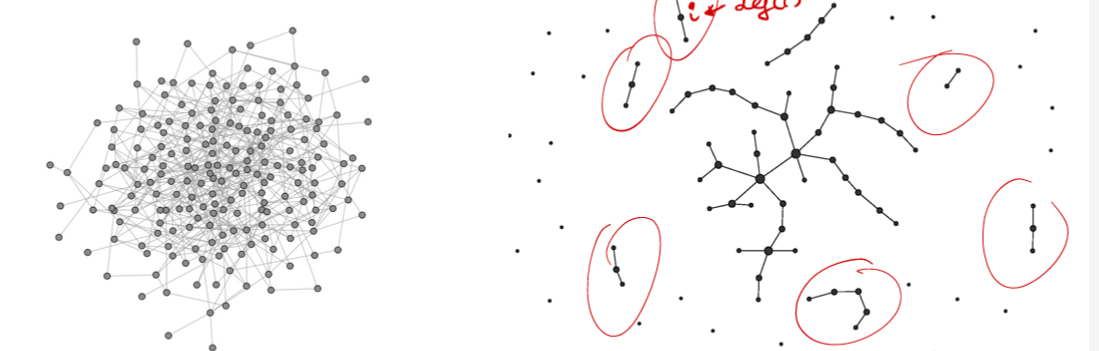
\includegraphics[width=\linewidth]{random-graph-phase-transition.png}
    \caption{Phase transitions of Erdos-Renyi random graph}
    \label{fig:random-graph-phase-transition}
\end{figure}

\begin{theorembox}
    There exists absolute constant $C > 0$, such that if $d \geq C\log(n)$, then $G(n,p)$ is almost $d$-regular with high probability. That means,
    \begin{equation*}
        \prob\left( \forall i, \text{deg}(i) : 0.9 d \leq d_i \leq 1.1 d \right) \geq 0.99
    \end{equation*}
\end{theorembox}
\begin{proof}
    Fix any $i$, let $E_i$ be the event that $\left|d_i - d\right| \leq \delta d$. Say $\delta \leq 1$. Then, by Chernoff inequality, we have
    \begin{equation*}
        \prob(E_i^c) \leq e^{-\delta^2 d/6} \leq e^{-\delta^2/6 \times C\log(n)} \leq \dfrac{1}{100n} ,
    \end{equation*}
    \noindent by choosing sufficiently large $C$. Now, union bound applies, i.e.,
    \begin{equation*}
        \prob\left( \bigcap_{i=1}^{N} E_i \right) \geq 1 - \sum_{i=1}^{n} P(E_i) \geq 1 - n\times \dfrac{1}{100n} = 0.99.
    \end{equation*}
\end{proof}

\begin{theorembox}[No regularity, but high degree clique]
    $\exists$ absolute constant $C > 0$ s.t. $d < C \log n$, the random graph $G(n, p)$ has a vertex with a large degree with high probability. These are called \textbf{hubs}. Mathematically,
    \begin{equation*}
        \prob\left( \exists i, \text{deg}(i) = d_i \geq 10d  \right) \approx 0.9.
    \end{equation*}
\end{theorembox}

\begin{proof}
    Since $d_i \sim \text{Binom}(n-1, p)$ with $\E(d_i) = d$, by application of reverse Chernoff inequality, we have
    \begin{align*}
        \prob(d_i \geq 10d)
         & \geq e^{-\mu} \left( \mu / t \right)^t, \ \text{ where } t = 10d \\
         & = e^{-d} (1/10)^{10d} \geq e^{-20d}                              \\
         & \geq e^{-20Clog(n)} \geq \dfrac{100}{n}
    \end{align*}
    \noindent by choosing sufficiently small $C$. Let, $E_i$ be the event that $d_i \geq 10d$ for any fixed $i$.

    Now if $E_i$s are independent, then it is possible that
    \begin{equation*}
        \prob\left( \cup_{i=1}^n E_i \right) = 1 - \prod_{i=1}^n \prob(E_i^c) = 1 - \left( 1 - \dfrac{100}{n} \right)^n \geq 1 - e^{-100} \geq 0.9.
    \end{equation*}
    \noindent But unfortunately, the above proof won't work since $E_i$s are not independent. Because if we have an edge between $i$ and $j$, then both $d_i$ and $d_j$ increases by one. However, for a fixed $i$ and $j$, if we ignore the edge between $i$ and $j$, the other edges of $i$ are independent of the other edges of $j$.

    So, we make some changes to the random graph $G(n, p)$ and create a new graph $G'$. In this new graph, we create two partitions of vertices, each of size $n/2$ vertices. Then we remove all the edges within the left partition, and within the right partition, but the edges remain between left and right partitions. At this point, if you pick two vertex $i$ and $j$ in the left partition, their modified degrees $\tilde{d}_i$ and $\tilde{d}_j$ are independently distributed. However, $\tilde{d}_i \sim \text{Binom}(n/2-1,p)$. It still holds that
    \begin{equation*}
        \dfrac{100}{n} \leq \prob(E_i) = \prob(d_i \geq 10d) = \prob(d_i / 2 \geq 5d) \leq \prob(\tilde{d}_i \geq 5d),
    \end{equation*}
    \noindent Now, we have
    \begin{equation*}
        \prob\left( \cup_{i=1}^n E_i \right) \geq \prob\left( \cup_{i \in \text{left half}} E_i \right) \geq 1 - \left( 1 - \dfrac{100}{n} \right)^{n/2} \geq 1 - e^{-50} \geq 0.9,
    \end{equation*}
    \noindent which completes the proof.
\end{proof}

\subsubsection{Discrepancy Theory}

Let's say we throw $N$ random points onto the 2d square $[0, 1]^2$, which are i.i.d. uniform points in $[0, 1]]^2$. Then, for all subset $I \subset [0, 1]^2$, the expected \# of points in $I$, $N_I \sim \text{Binom}(N, \lambda_I)$, where $\lambda_I$ is the area of $I$. Clearly,
\begin{align*}
    \E N_I         & = N\lambda_I                           \\
    \var(N_I)      & = N\lambda_I(1-\lambda_I) < N\lambda_I \\
    \text{sd}(N_I) & \leq \sqrt{N\lambda_I}
\end{align*}
\noindent Therefore, by Chebyshev's inequality this means, $N_I \approx N\lambda_I \pm C\sqrt{N\lambda_I}$ with high probability.

\begin{note}
    However, once the points are given, it is possible to choose a subset $I'$ such that $N_{I'} = 0$. Therefore, the above result holds only if the set is chosen predefined, and then the points are randomly distributed.
\end{note}

However, when we perform statistical methodologies, we choose the random sample first, and then analyze the data using different models. It is not that we fix the entire inference procedure beforehand, even before collecting the data. This identifies a core problem in all of statistical studies that we do currently.

This means we want some kind of result that holds regardless of the procedure used (or simultaneously for all nice classes of procedures). In the above example, it means to establish a result that is true for all nice sets $I$ simultaneously. Usually we take this class of nice sets as the convex sets, or Euclidean balls or rectangles, etc.

\begin{theorembox}
    A set of $N$ i.i.d. uniform random points on $[0, 1]^2$ satisfies the following with probability at least $0.99$ (or any $1-\epsilon$ for a given $\epsilon > 0$): For all axis-aligned rectangle $I$, we have
    \begin{equation*}
        \lambda_I N - C\sqrt{\lambda_I N \log(N)} \leq N_I \leq \lambda_I N + C\sqrt{\lambda_I N \log(N)}
    \end{equation*}
    \noindent for an absolute constant $C$ and sufficiently large $N$.
\end{theorembox}

\begin{note}
    \begin{enumerate}
        \item We lose a $\sqrt{\log(N)}$ factor to establish the uniform bound.
        \item Simple union bound may not be possible since there are infinite \# of rectangles. The idea is similar to $\epsilon$-nets and we consider $\epsilon$-grid lines and the rectangles generated by them alone.
    \end{enumerate}
\end{note}

\begin{proof}
    We use an $\epsilon$-net argument, by considering $\epsilon$-grid lines over $[0, 1]^2$ and the rectangles generated by them. We call these \textbf{net rectangles}.

    \textbf{Step 1 (Concentration):} Fix any net rectanlge $I$, with area $\lambda_I$. Then, as $N_I \sim \text{Binom}(N, \lambda_I)$, by Chernoff's inequality, we have
    \begin{align*}
                 & \prob\left( \vert N_I - \lambda_I N\vert \geq \delta \lambda_I N \right) \leq 2 e^{-\delta^2 \lambda_I N/6}                                                                            \\
        \implies & \prob\left( \vert N_I - \lambda_I N\vert \geq \lambda_I N \times C \dfrac{\sqrt{\log N}}{\sqrt{\lambda_I N}} \right) \leq 2 \exp\left[ - C^2 \log N/6 \right] \leq \dfrac{1}{N^{100}},
    \end{align*}
    \noindent for sufficiently large $C$ and $N$. Here we choose $\delta = C \dfrac{\sqrt{\log N}}{\sqrt{\lambda_I N}}$.

    \textbf{Step 2 (Union Bound):} Let $B_I$ be the event that rectangle $I$ is bad, i.e., the number of points does not fall within the required bound, i.e., $\vert N_I - \lambda_I N\vert \geq C \sqrt{\lambda_I N \log(N)}$. Now,
    \begin{equation*}
        \prob(\exists \text{ a bad } I) = \prob(\cup B_I ) \leq \sum_I \prob(B_I) \leq \left( \dfrac{1}{\epsilon} \right)^8 \dfrac{1}{N^{100}}.
    \end{equation*}
    \noindent By choosing $\epsilon = 1/N^{10}$, we have the probability that there is a bad net rectangle $I$ to be less than $\dfrac{1}{N^{20}}$, which can be made smaller than $0.99$ by choosing sufficiently large $N$.

    \textbf{Step 3 (Approximation):} This result so far holds for uniformly with high probability, but only for net rectangles. We need to show now that the number of points in any rectangle can be approximated well by the number of points in the net rectangle. Let $J$ be another rectangle, then there is a net rectangle $I$ (slightly smaller) such that
    \begin{equation*}
        \lambda_J \leq \lambda_I \leq \lambda_J + \dfrac{4}{\epsilon} = \lambda_J + \dfrac{4}{N^{10}}.
    \end{equation*}
    \noindent Therefore,
    \begin{align*}
        N_J \leq N_I
         & \leq \lambda_I N + C\sqrt{\lambda_I N \log(N)}, \ \text{ since } I \text{ is good }                                                                                     \\
         & \leq \left( \lambda_J + \dfrac{4}{N^{10}} \right)N + C\left( \left( \lambda_J + \dfrac{4}{N^{10}} \right) N \log(N) \right)^{1/2}                                       \\
         & \leq \lambda_J N + C \sqrt{\lambda_J N \log(N)} + \left( \dfrac{4}{N^9} + C \dfrac{\sqrt{4\log(N)}}{N^9} \right), \ \text{since } \sqrt{a + b} \leq \sqrt{a} + \sqrt{b} \\
         & \leq \lambda_J N + 2 C\sqrt{\lambda_J N \log(N)}, \text{ since the second term is smaller than } \sqrt{\lambda_J N \log(N)}
    \end{align*}
    \noindent This means, we only lose a factor of $2$.
\end{proof}


\subsection{Spaces of Random Variables}

\begin{definitionbox}
    A \textbf{normed space} is a vector space $M$ over field $F$ that is equipped with a norm $\norm{\cdot}$. The norm $\norm{\cdot} : M \rightarrow \R$ is a function such that
    \begin{enumerate}
        \item $\norm{x} \geq 0$ for all $x \in M$ with equality if and only if $x = 0$.
        \item $\norm{\alpha x} = \abs{\alpha}\norm{x}$ for all $\alpha \in F$ and $x \in M$.
        \item $\norm{x + y} \leq \norm{x} + \norm{y}$ for all $x, y \in M$.
    \end{enumerate}
    \noindent i.e., it has a measure of length.
\end{definitionbox}

\begin{definitionbox}
    A \textbf{Hilbert} space is a vector space $H$ over field $F$ equipped with an inner product, $\inner{\cdot,\cdot} : H \times H \rightarrow \R$ such that
    \begin{enumerate}
        \item $\inner{x, x} \geq 0$ for all $x \in H$ with equality if and only if $x = 0$.
        \item $\inner{x, y} = \inner{y, x}$ for all $x, y \in H$.
        \item $\inner{ax + by, z} = a\inner{x, z} + b\inner{y, z}$, where $a, b\in F$ and $x, y, z \in H$.
    \end{enumerate}
    \noindent i.e., it has a measure of angle, which in turn, defines length.
\end{definitionbox}

Clearly, a Hilbert space is a normed space with $\norm{x} = \sqrt{\inner{x, x}}$. We immediately have the Cacuhy-Schwartz inequality,
\begin{equation*}
    \vert \inner{x,y} \vert \leq \norm{x}\norm{y}
\end{equation*}
\noindent In case of $L^2$ space of random variables, this converts into $\vert \E(XY)\vert \leq (\E X^2)^{1/2} (\E Y^2)^{1/2}$. We also have a more general H\"{o}lder's inequality,
\begin{equation*}
    \vert \E(XY)\vert \leq \left( \E\abs{X}^p \right)^{1/p} \left( \E\abs{X}^q \right)^{1/q} = \norm{X}_{L^p} \norm{X}_{L^q},
\end{equation*}
\noindent where $(1/p + 1/q) = 1$ for some $p, q \geq 0$.

A more general is the \textbf{Jensen's} inequality, which says:
\begin{theorembox}[Jensen's inequality]
    Let $X$ be a real-valued random variable and $\phi: \R \rightarrow \R$ be a convex function. Then,
    \begin{equation*}
        \phi(\E(X)) \leq \E(\phi(X)).
    \end{equation*}
\end{theorembox}
\noindent A fact that follows from the above is that the $L^p$ norm $\norm{X}_{L^p}$ is an increasing function of $p$ for all $p \geq 1$. Before, we show the proof for this fact.

\begin{proof}
    We will show that if $p \leq q$, then $\norm{X}_{L^p} \leq \norm{X}_{L^q}$. If $p < q$, choose a function $\phi(x) = x^{q/p}$, is convex as $q > p$ or $q/p > 1$.

    By applying Jensen's inequality on this function with random variable $\abs{X}^p$,
    \begin{align*}
         & \phi(\E\abs{X}^p) \leq \E(\phi(\abs{X}^p))                \\
        \implies \left( \E\abs{X}^p \right)^{q/p} \leq \E(\abs{X}^q) \\
        \implies \norm{X}^{L^p} \leq \norm{X}_{L^q}
    \end{align*}
    \noindent where the last line follows from taking $p$-th root from both sides, and since $p \geq 1$.
\end{proof}

As a result of this, we have
\begin{equation*}
    \lim_{p \to \infty} \norm{X}_{L^p} = \norm{X}_{L^\infty} =: \text{essential supremum of } |X|.
\end{equation*}
\noindent The essential supremum is the supremum of a random variable over a set of probability $1$ discarding the set of measure zero. Also, we have,
\begin{equation*}
    L^1 \supset L^2 \supset \dots \supset L^\infty,
\end{equation*}
\noindent where $L^k$ is the space having finite $k$-th order moment and the $L^\infty$ is the space of random variables that are bounded almost surely.

\begin{note}
    Note that, $\cap_{p \geq 1} L^p \neq L^\infty$, since there are random variables (e.g. $N(0,1)$) that has finite moments for all order but still is not bounded.
\end{note}

This means, there must exists special kinds of norms that we can bound so that the resulting spaces remain in this gap. In general, we understand that $L^p$ spaces look at the $p$-th moment by considering the function $x^p$. But we could look at finite expectation of different moments like $e^x$, or $\sin(x^2)$, or something like this.

\begin{definitionbox}[Orlicz Functions]
    A function $\psi: \mathbb{R}^+ \to \mathbb{R}^+$ is called an \textbf{Orlicz function} if it is convex, increasing, and,
    \begin{equation*}
        \psi(x) \to
        \begin{cases}
            0,      & \text{as } x \to 0      \\
            \infty, & \text{as } x \to \infty
        \end{cases}
    \end{equation*}
    \noindent e.g. $\psi(x) = x^p$ or $\psi(x) = e^x - 1$.
\end{definitionbox}

\begin{definitionbox}[Orlicz norm]
    For a given Orlicz function $\psi$, the Orlicz ``norm'' of a random variable $X$ is defined as
    \begin{equation*}
        \norm{X}_{\psi} = \inf\left\{ k > 0: \E[\psi(\abs{X}/k)] \leq 1 \right\}
    \end{equation*}
\end{definitionbox}

To ensure that this definition is valid, we need to show the resulting quantity indeed defines a norm. Following is the justification for this.

\begin{enumerate}
    \item Clearly, $\norm{X}_{\psi} \geq 0$ for any random variable $X$, because it is infinimum of a set with positive quantities.
    \item If $X \equiv 0$ almost surely, then by definition of Orlicz function, $\psi(\abs{X}/k) = \psi(0) \equiv 0$ almost surely for any choice of $k > 0$. Therefore, the Orlicz norm is zero. Conversely, suppose that that Orlicz norm is $0$ but $X$ is not equal to $0$ almost surely. Then, for any $k > 0$, we must have $\E(\psi(\abs{X}/k)) \leq 1$. And since it is not true that $X$ is zero almost surely, there exists $\epsilon > 0$ such that $\abs{X} > \epsilon$ with probability at least $\delta$ for some $\delta > 0$. Also, since the Orlicz function is increasing, convex and $\psi(x) \to \infty$ as $x \to \infty$, there exists $M > 0$ such that $\psi(x) > 1/\delta$ for all $x \geq M$. Therefore, by choosing $k = \epsilon /M$, we have
          \begin{equation*}
              \E(\psi(\abs{X}/k)) = \int \psi(\abs{X}M/\epsilon)dP(x) \geq \int_{\abs{x} > \epsilon} \psi(\abs{x}M/\epsilon)dP(x) \geq \psi(M)\delta \geq 1 > 0.
          \end{equation*}
          \noindent This leads to a contradiction.
    \item The linearity of the Orlicz norm is trivial.
    \item For the triangle inequality, we need to know that for any two random variables $X$ and $Y$, $\norm{X + Y}_\psi \leq \norm{X}_\psi + \norm{Y}_\psi$. By definition of Orlicz norm, it is enough to show that for $k = \norm{X}_\psi + \norm{Y}_\psi$,
          \begin{equation*}
              \E\psi(\abs{X + Y}/k) \leq 1.
          \end{equation*}
          \noindent To see this, note that
          \begin{align*}
                         & \E\psi(\abs{X + Y}/k)                                                                                                                                                                                                                                       \\
              \leq \quad & \E\psi(\abs{X}/k + \abs{Y}/k), \text{ since } \psi \text{ is increasing }                                                                                                                                                                                   \\
              = \quad    & \E\psi\left( \dfrac{\abs{X}}{\norm{X}_\psi} \dfrac{\norm{X}_\psi}{\norm{X}_\psi + \norm{Y}_\psi} + \dfrac{\abs{Y}}{\norm{Y}_\psi} \dfrac{\norm{Y}_\psi}{\norm{X}_\psi + \norm{Y}_\psi} \right)                                                              \\
              = \quad    & \dfrac{\norm{X}_\psi}{\norm{X}_\psi + \norm{Y}_\psi} \E\psi\left( \dfrac{\abs{X}}{\norm{X}_\psi} \right) + \dfrac{\norm{Y}_\psi}{\norm{X}_\psi + \norm{Y}_\psi} \E\psi\left( \dfrac{\abs{Y}}{\norm{Y}_\psi} \right), \text{ since } \psi \text{ is convex } \\
              \leq \quad & \dfrac{\norm{X}_\psi}{\norm{X}_\psi + \norm{Y}_\psi} + \dfrac{\norm{Y}_\psi}{\norm{X}_\psi + \norm{Y}_\psi} = 1.
          \end{align*}
          \noindent The last inequality follows from the definition of $\norm{X}_\psi$ and $\norm{Y}_\psi$.
\end{enumerate}

Now that we know that it is indeed a well-defined norm, we can define the Orlicz space as follows.

\begin{equation*}
    L_\psi = \left\{ X: \norm{X}_\psi < \infty \right\}
\end{equation*}

To illustrate further, consider the following examples.

\begin{enumerate}
    \item If $\psi(x) = x^p$, then $\E[\psi(|X|/k)] = \E[(|X|/k)^p] \leq 1 \implies k \geq (\E[|X|^p])^{1/p}$ and $\norm{X}_\psi = \norm{X}_p$.
    \item If $\psi(x) = e^x - 1$, then $\E\psi(|X|/k) = \E[e^{|X|/k} - 1] \leq 1 \implies \E[e^{\abs{X}/k}] \leq 2$, which is something related to the MGF of a random variable.
\end{enumerate}

Now turning our attention to the Hoeffding's inequality, we note that if $X_i$s are i.i.d. symmetric Bernoulli random variables, then $\bar{X}_n = \sum_{i=1}^n X_i / n$ has Gaussian tails. The same thing holds if $X_i$ are i.i.d. standard normal random variables. Also, you can verify that if $X_i$ are i.i.d. uniform random variables on $[-1/2,1/2]$, then also $\bar{X}_n$ has Gaussian tails.

\textbf{Hence, the question is to find out the biggest class of distributions for which we have Gaussian tails.}

Turns out, if $n = 1$, then $\bar{X}_n = X_1$ needs to satisfy,
\begin{equation*}
    \prob(\abs{X_1} \geq t) \leq 2e^{-ct^2/2}, \forall t > 0.
\end{equation*}
\noindent since the above needs to be true for all choices of $n$. Therefore, this is a necessary condition. Turns out this is also sufficient for the Hoeffding lemma to hold. The random variables which has tails satisfying the above inequality are called \textbf{sub-Gaussian random variables}.


\subsubsection{Sub Gaussian Random Variables}

Before we look at the general behaviour of them, let us look at the special case for $X_i \sim N(0, 1)$. In this case,
\begin{enumerate}
    \item \textbf{Tails:} We have $\prob(|X_i| \geq t) \leq 2e^{-t^2/2}$, $\forall t > 0$.
    \item \textbf{Moments:} $\E(X_i^p) = 0$ if $p$ is odd and is equal to $(p-1)!!$ if $p$ is even. This means that the $L^p$ norm of the Gaussian random variable satisfy
          \begin{equation*}
              \norm{X_i}_p = \left( \E(\abs{X_i}^p) \right)^{1/p} \leq \left( (p-1)(p-3)\dots 5\times 3 \times 1 \right)^{1/p} \leq (p^{p/2})^{1/p} = \sqrt{p}
          \end{equation*}
          \noindent for all $p \geq 1$.
    \item \textbf{MGF:} The MGF of $X_i$ is given by $\E(e^{tX_i}) = e^{t^2/2}$.
    \item \textbf{MGF of square:} The MGF of $X_i^2$ is given by $\E(e^{tX_i^2}) = \dfrac{1}{\sqrt{1-2t}}$, if $t < 1/2$. Otherwise it is infinite. Therefore, if we take the Orlicz function $\psi_2(x) = e^{x^2} -1$, then
          \begin{align*}
                       & \E\psi(\abs{X_i}/k) \leq 1                  \\
              \implies & \E\left[ e^{X_i^2/k^2} \right] \leq 2       \\
              \implies & \dfrac{1}{\sqrt{1 - 2 \times 1/k^2}} \leq 2 \\
              implies  & k \geq \sqrt{2}.
              \implies & \norm{X_i}_{\psi_2} \leq \sqrt{2}.
          \end{align*}
\end{enumerate}

The following lemma establishes that this connection between the finiteness of all these quantities is not special for Gaussian random variables, but for all sub-Gaussian random variables.

\begin{lemma}[sub-Gaussian Lemma]
    For all random variable $X$, the following the equivalent.
    \begin{enumerate}
        \item $\exists K_1$ such that $\prob(\abs{X} \geq t) \leq 2 e^{-t^2/K_1^2}$, for all $t > 0$.
        \item $\exists K_2$ such that $\norm{X}_p \leq K_2 \sqrt{p}$, for all $p \geq 1$.
        \item $\exists K_3$ such that $\E\exp(X^2/K_3^2) \leq 2$.
        \item If $\E(X) = 0$, then $\exists K_4$ such that $\E\exp(\lambda X) \leq e^{\lambda^2 K_4^2}$, for all $\lambda \in \mathbb{R}$.
    \end{enumerate}
    \noindent These constants $K_1, \dots, K_4$, are all equivalent to the sub-Gaussian norm $\norm{X}_{\psi_2}$.
\end{lemma}

\begin{proof}
    \textbf{$(1) \implies (2)$:} Without loss of generality, assume that $K_1 = 1$. Then,
    \begin{align*}
        \E\abs{X}^p
         & = \int_{0}^\infty \prob(\abs{X}^p > t) dt                                                \\
         & = \int_{0}^\infty \prob(\abs{X} > s) p s^{p-1} ds,\  \text{ by substitution of } t = s^p \\
         & \leq \int_{0}^\infty 2e^{-s^2} ps^{p-1} ds                                               \\
         & = p(p/2 - 1)! \ \text{ as it is Gamma integral }                                         \\
         & \leq p p^{p/2 - 1} = p^{p/2}.
    \end{align*}
    \noindent Therefore, $\norm{X}_{L^p} \leq \sqrt{p}$.

    \textbf{$(2) \implies (3)$:} Without loss of generality, assume $K_2 = 1$. Then,
    \begin{align*}
        \E(e^{X^2/100})
         & = \E\left( \sum_{p=0}^\infty \dfrac{(X^2/100)^p}{p!} \right)   \\
         & = \sum_{p=0}^\infty \dfrac{1}{p! (100)^p} \E(X^{2p})           \\
         & \leq \sum_{p=0}^\infty \dfrac{1}{p! (100)^p} (2p)^{p}          \\
         & \text{ since by Stirling's approximation } p! \geq e^{-p}p^p   \\
         & \leq \sum_{p=0}^\infty \dfrac{(2p)^p}{(100)^p (p/e)^p}         \\
         & = \sum_{p=0}^{\infty} \left( \dfrac{2e}{100} \right)^p \leq 2.
    \end{align*}

    \textbf{$(3) \implies (4)$:} Without loss of generality, assume that $K_3 = 1$. We know that $e^x \leq x + e^{x^2}$ for all $x \in \R$. Therefore,
    \begin{align*}
        \E(e^{\lambda X})
         & \leq \E(\lambda X) + \E(e^{\lambda^2 X^2})                                           \\
         & = 0 + \left( \E(e^{X^2}) \right)^{\lambda^2}, \ \text{ assume } \abs{\lambda} \leq 1 \\
         & \leq 2^{\lambda^2} = e^{\lambda^2 \log(2)}.
    \end{align*}

    \textbf{$(4) \implies (1)$:} Without loss of generality, assume that $K_4 = 1$. Then,
    \begin{align*}
        \prob(\abs{X} \geq t)
         & = \prob(e^{\lambda \abs{x}} \geq e^{\lambda t})                               \\
         & \leq e^{-\lambda t} \E(e^{\lambda \abs{X}}), \ \text{ by Markov's inequality} \\
         & \leq e^{-\lambda t} e^{\lambda^2}                                             \\
         & = e^{-\lambda t + \lambda^2}
    \end{align*}
    \noindent Optimizing over $\lambda$, we get $\lambda = t/2$, yielding the bound $e^{-t^2/4}$.
\end{proof}

\begin{lemmabox}
    If $X_i$s are independent mean zero sub-Gaussian random variables, then $\norm{\sum_i X_i}_{\psi_2} \leq C \sum_{i=1}^n \norm{X_i}_{\psi_2}$ for some absolute constant $C$.
\end{lemmabox}

\begin{proof}
    We will make use of the sub-Gaussian Lemma. Note that,
    \begin{align*}
        \E(e^{\lambda \sum_i X_i})
         & = \prod_{i=1}^n \E(e^{\lambda X_i}), \ \text{ by independence } \\
         & \leq \prod_{i=1}^n e^{C \norm{X_i}_{\psi_2}^2 \lambda_i^2}      \\
         & = e^{C \sum_i \norm{X_i}_{\psi_2}^2 \lambda_i^2}.
    \end{align*}
    \noindent By equivalence of the sub-Gaussian properties, we get that $\sum_{i} X_i$ is also a sub-Gaussian random variable and that
    \begin{equation*}
        \norm{\sum_i X_i}_{\psi_2} \leq C' \sum_{i=1}^n \norm{X_i}_{\psi_2}
    \end{equation*}
    \noindent for some constant $C'$.
\end{proof}

As a result, the Hoeffding's inequality follows for sub-Gaussian random variables as well, because the tail behaviour indicates Gaussianity.

\begin{theorembox}[Hoeffding's inequality for sub-Gaussian random variables]
    If $X_i$ are independent mean zero sub-Gaussian random variables, then
    \begin{equation*}
        \prob\left(\abs{\sum_i X_i} \geq t\right) \leq 2e^{-C t^2/\sigma^2}
    \end{equation*}
    \noindent where $\sigma^2 = \sum_{i=1}^n \norm{X_i}_{\psi_2}^2$. This $\sigma^2$ is kind of a proxy for the variance.
\end{theorembox}

However, it turns out that the sub-Gaussian class is not large enough to capture all kind of random variables that we usually deal with. For example, if $X$ is sub-Gaussian, then $X^2$ is not sub-Gaussian.
\begin{equation*}
    \prob(X^2 \geq t) = \prob(\abs{X} \geq \sqrt{t}) \asymp e^{-c(\sqrt{t})^2} = e^{-ct} >> e^{-ct^2}, \ \forall t > 0.
\end{equation*}
\noindent The tail in this case is heavier than the Gaussian case, but it still decays exponentially. We call this a \textbf{sub-exponential} random variable.

\subsubsection{Sub-exponential Random Variables}

A similar lemma as before can be stated for sub-exponential random variables.

\begin{lemma}[sub-exponential Lemma]
    For all random variable $X$, the following the equivalent.
    \begin{enumerate}
        \item $\exists K_1$ such that $\prob(\abs{X} \geq t) \leq 2 e^{-t/K_1}$, for all $t > 0$.
        \item $\exists K_2$ such that $\norm{X}_{L^p} \leq K_2 p$, for all $p \geq 1$.
        \item $\exists K_3$ such that $\E\exp(\abs{X}/K_3) \leq 2$.
        \item $\exists K_4$ such that $\E\exp(\lambda X) \leq e^{\lambda^2 K_4^2}$, for all $\abs{\lambda} \leq 1/K_4$.
    \end{enumerate}
    \noindent These constants $K_1, \dots, K_4$, are all equivalent to the sub-exponential norm $\norm{X}_{\psi_1}$.
\end{lemma}

A particular thing to note that is the last bound on the MGF does not hold for all $\lambda$, because the MGF may not converge for all $\lambda$. To understand this, note that
\begin{equation*}
    \E(e^{\lambda X})= \int_0^\infty e^{\lambda x} p(x)dx \asymp \int_0^\infty e^{\lambda x}e^{-cx} dx
\end{equation*}
\noindent so the integral converges if and only if $\lambda < c$.

Clearly, Hoeffding's inequality does not hold for sub-exponential random variables in general. Since if $n = 1$, we cannot have $\prob(\abs{X} \geq t) \leq e^{-ct^2}$. However, once we accumulate multiple independent $X_i$s, we can still obtain a Gaussian tail behaviour.

\begin{theorembox}[Bernstein's inequality]
    Let $X_i$s are independent mean zero sub-exponential random variables. Then,
    \begin{equation*}
        \prob\left( \abs{\sum_{i=1}^n X_i} \geq t  \right) \leq 2\exp\left[ - C\min\left\{ \dfrac{t^2}{\sigma^2}, \dfrac{t}{K} \right\} \right]
    \end{equation*}
    \noindent where $\sigma^2 = \sum_{i=1}^n \norm{X_i}_{\psi_1}^2$ and $K = \max_{i=1}^n \norm{X_i}_{\psi_1}$.
\end{theorembox}

\subsection{Applications: Part 2}

\subsubsection{Thin Shell Phenomenon}

Consider a Gaussian random vector $g \sim N(0, I_n)$. We expect the samples from this $N(0, I_n)$ to look like the left one, but the actual picture looks like the right one in a high-dimensional space.

\begin{figure}[h]
    \centering
    \begin{tikzpicture}
        \draw (-1.5, -1.5) rectangle (1.5, 1.5);
        \node at (0.9, 0) {$0 \in \R^n$};
        \node at (0, 0) {$\circ$};
        \foreach \Point in {(0.1, 0.4), (-0.1, 0.2), (-0.2, -0.1), (-0.2, -0.4), (0.5, 0.7), (0.2, 0.2), (-0.4, -0.8), (-0.4, 0.1), (0, -0.3), (-0.7, -0.2), (0.3, -0.4)}{
                \node at \Point {\textbullet};
            }

        \draw (10, 0) circle (1.5);
        \draw[dotted] (10, 0) circle (1);
        \foreach \Point in {(10.5, 0.6), (9.7, -0.8), (10.2, -1), (9, -0.1), (9.4, 0.5)}{
                \node at \Point {\textbullet};
            }
    \end{tikzpicture}
\end{figure}


This means the samples concentrate on a thin ring close the to boundary of a the $\sqrt{n}$-ball, instead of concentrating near zero. The next theorem establishes this fact.

\begin{theorembox}
    For $g \sim N(0, I_n)$, $\prob(0.99\sqrt{n} \leq \norm{g}_2 \leq 1.01\sqrt{n}) \geq 1 - 2e^{-cn}$, for some sufficiently small but absolute constant $c$.
\end{theorembox}

\begin{proof}
    Note that,
    \begin{equation*}
        \norm{g}_2^2 - n
        = \sum_{i=1}^n (g_i^2 - 1)
        = \sum_{i=1}^n (g_i^2 - \E(g_i^2))
    \end{equation*}
    \noindent Since the above is a sum of i.i.d. terms, we can apply concentration inequalities. In particular, $g_i$ is sub-Gaussian, so $g_i^2$ is only sub-exponential, hence we need to apply Bernstein's inequality. Using that, we get
    \begin{equation*}
        \prob\left( \vert \norm{g}_2^2 - n\vert \geq 0.01n \right) \leq 2 \exp\left[ - c\min\left( \dfrac{n^2}{\sigma^2}, \dfrac{n}{K} \right) \right]
    \end{equation*}
    \noindent where
    \begin{align*}
        \sigma^2 & = \sum_{i=1}^n \norm{g_i^2 - 1}_{\psi_1} \leq nC                                            \\
        K        & = \max_{i} \norm{g_i^2 - 1}_{\psi_1} = \norm{g_1^2 - 1}_{\psi_1} (\text{ as i.i.d.}) \leq C
    \end{align*}
    \noindent Therefore, we have
    \begin{equation*}
        \prob\left( 0.99n \leq \norm{g}_2^2 - n \leq 1.01n \right) \geq 1 - 2e^{-c' n}
    \end{equation*}
    \noindent for some $c'$. Now, note that
    \begin{equation*}
        \dfrac{\norm{g}_2 - \sqrt{n}}{\sqrt{n}} = \dfrac{\norm{g}_2^2 - n}{\sqrt{n}(\norm{g}_2 + \sqrt{n})} = \dfrac{\leq 0.01n}{\geq \sqrt{n} \times \sqrt{n}} \leq 0.01n,
    \end{equation*}
    \noindent Therefore, the result follows.
\end{proof}



\pagebreak
\sr{CHECK FROM HERE}




\textbf{Thin Shell Phenomenon:}

Proof: Consider, $\|g\|_2^2 - n = \sum_{i=1}^n (g_i^2 - 1)$ \hspace*{2cm} $g_i =$ coordinate of $g$
\hspace*{4cm} $= \sum_{i=1}^n (g_i^2 - \E g_i^2) \longrightarrow$ sum of iid terms

$g_i^2$ is sub-exponential

So, we apply Bernstein's ineq., $\prob(|\|g\|_2^2 - n| \geq 0.01 n) \leq 2e^{-c \min(\frac{n^2}{\sigma^2}, \frac{n}{K})}$

$\sigma^2 = \sum_{i=1}^n \|g_i^2 - 1\|_{\psi_1} \leq n C$, and, $K = \max_i \|g_i^2 - 1\|_{\psi_1} = \|g_1^2 - 1\|_{\psi_1} \leq C$
\hspace*{8cm} $\uparrow$
\hspace*{8cm} Since iid

Therefore, $\prob(0.99 n \leq \|g\|_2^2 \leq 1.01 n) \geq 1 - 2e^{-c \min(\frac{n^2}{Cn}, \frac{n}{C})} \geq 1 - 2e^{-cn}$
\hspace*{2cm} $\underbrace{\text{take square root now,}}$
\hspace*{2cm} \& get another constant

\section*{Dimension Reduction}

Let $x_1, x_2, \ldots, x_N \in \mathbb{R}^n$ be given map to $\mathbb{R}^m$, $m \ll n$
where we preserve the pairwise distances (approximately)
Is it possible with $m = O(\log N)$?

\textbf{Thm} (Johnson - Lindenstrauss lemma, 1984) $\forall x_1, \ldots, x_N \in \mathbb{R}^d$, $\exists$ a linear map $T$:
$T: \mathbb{R}^d \to \mathbb{R}^m$, such that, $m < C \log N$, and,
$0.99 \|x_i - x_j\|_2 \leq \|T(x_i) - T(x_j)\|_2 \leq 1.01 \|x_i - x_j\|_2, \forall i,j=1,2,\ldots,N$

\textbf{Proof:} Choose a random map, say, matrix corresponding to $T$ is, $G_i$, with $G_{ij} \stackrel{iid}{\sim} N(0,1)$

$m \begin{bmatrix} G \end{bmatrix}_d = \begin{bmatrix} I \end{bmatrix}_m$ \hspace{2cm} Fix any $z \in \mathbb{R}^d$, s.t. $\|z\|_2 = 1$.

\hspace{4cm} Then, $Gz \sim N(0,I_m)$, as, $(Gz)_i = \sum_{j=1}^d G_{ij} z_j$
\hspace{7cm} $\sim N(0, \sum_{j=1}^d z_j^2) = N(0,1)$

By thin shell theorem:
$\prob(0.99 \sqrt{m} \leq \|Gz\|_2 \leq 1.01 \sqrt{m}) \geq 1 - 2e^{-cm}$ \hspace{2cm} (1)

Now for any $i,j$, using (1), we have, $\prob(0.99 \sqrt{m} \leq \|G(\frac{x_i-x_j}{\|x_i-x_j\|_2})\|_2 \leq 1.01 \sqrt{m}) \geq 1 - 2e^{-cm}$

$\Rightarrow \prob(0.99 \sqrt{m} \|x_i-x_j\|_2 \leq \|T(x_i)-T(x_j)\|_2 \leq 1.01 \sqrt{m} \|x_i-x_j\|_2) \geq 1 - 2e^{-cm}$

$\Rightarrow$ By union $\forall i,j$ pairs,
bound, \hspace{4cm} where, $T = \frac{1}{\sqrt{m}} G$.

$\prob(\forall i,j, 0.99 \|x_i-x_j\|_2 \leq \|T(x_i)-T(x_j)\|_2 \leq 1.01 \|x_i-x_j\|_2) \geq 1 - 2N^2e^{-cm}$
\hspace{7cm} $= 1 - 2\exp(-cm+2\log N)$

Choose $cm = 4\log N$, so to get, $\geq 1 - 2\exp(-2\log N) = 1 - \frac{2}{N^2} > 0$, if $N \geq 2$

$\Rightarrow m = \frac{4}{c}\log N = O(\log N)$.

$\Rightarrow \exists$ a map for which this holds deterministically.

\textbf{Obs:}
$\Rightarrow$ The std $\sigma(X)$ captures only "2nd moment" \& average spread, while Sub-Gaussian
norm captures all moments, MGF, etc. This exercise shows Sub-Gauss.
norm dominates $\sigma(X)$ but not other way around.

$\Rightarrow$ Let, $X$ be sub-gaussian, \& assume $\E X = 0$. WLOG.
\hspace{7cm} $\to$ absolute
Then, $\sigma(X) = (\E X^2)^{1/2} = \|X\|_2 \leq \sqrt{2} K_2 \|X\|_{\psi_2} \leq C \|X\|_{\psi_2}$

$\Rightarrow$ Let, $X \sim N(\mu, \sigma^2)$, then, $\sigma(X) = \sigma$, and, let $\|X\|_{\psi_2} = K$ \hspace{1cm} (*)

Then, $\E(e^{X^2/K^2}) \leq 2 \Rightarrow \int_{-\infty}^{\infty} \frac{1}{\sqrt{2\pi}\sigma} e^{x^2/K^2} \cdot e^{-x^2/2\sigma^2} dx < 2 \Rightarrow \frac{\sigma^2}{K^2} < \frac{1}{2\sigma^2}$
\hspace{8cm} $\Rightarrow K^2 > 2\sigma^2$

$\Rightarrow K = \sqrt{2}\sigma$ works.

$\Rightarrow \|X\|_{\psi_2} \leq \sqrt{2}\sigma = 4$ \hspace{1cm} $\boxed{\|X\|_{\psi_2} \leq C \sigma(X)}$ $\to$ in this case reverse
\hspace{5cm} $\uparrow$ (*) \hspace{2cm} inequality holds

$\Rightarrow$ But consider, $X \sim Poisson(\lambda)$
$\|X\|_{\psi_2} = \infty$, as it is not sub-gaussian
\hspace{3cm} So, we do not have (*).
But, $Var(X) = \lambda \Rightarrow \sigma(X) = \sqrt{\lambda} < \infty$,



\end{document}


\textbf{Homework:}

\textbf{Q1:} \text{Let, } X_1, X_2, \dots, X_N \text{ be non-negative i.i.d. r.v. Assume PDF of each } X_i \text{ is uniformly bounded by } 1.
\begin{enumerate}[a)]
    \item \text{Show that } \prob(X_i < \epsilon) \leq \epsilon, \forall \epsilon > 0.

          \text{Follows from, } \prob(X_i < \epsilon) = \int_0^\epsilon f(x) dx \leq \epsilon \cdot \left(\sup_x f(x) \leq 1\right)

    \item \text{Show that MGF of each } X_i \text{ satisfies, } \E \left[e^{-tX_i}\right] \leq \frac{1}{t}, \forall t > 0.

          \text{To see this, } \E \left[e^{-tX_i}\right] = \int_0^\infty e^{-tx} f(x) dx \leq \frac{1}{t}

    \item \text{Deduce that averaging increases the strength of (a) exponentially, i.e. }

          \prob\left(\frac{1}{N}\sum_{i=1}^N X_i < \epsilon\right) \leq (c\epsilon)^N, \forall \epsilon > 0.

          \text{To see this, }
          \begin{align*}
              \prob\left(\frac{1}{N}\sum_{i=1}^N X_i < \epsilon\right) & = \prob\left(e^{-\frac{t}{N}\sum_{i=1}^N X_i} > e^{-tN\epsilon}\right)                    \\
                                                                       & \leq e^{-tN\epsilon} \E\left[e^{-\frac{t}{N}\sum_{i=1}^N X_i}\right]                      \\
                                                                       & = e^{-tN\epsilon} \left(\E\left[e^{-\frac{t}{N}X_i}\right]\right)^N \quad \text{(Markov)} \\
                                                                       & \leq e^{-tN\epsilon} \left(\frac{1}{t}\right)^N
          \end{align*}

          \text{Now, we optimize over } t > 0, \text{ setting:} \quad e^{LNE} = \exp\left(-tN\epsilon - N\log t\right)

          \Rightarrow \frac{\partial (\text{bound})}{\partial t} = -NE - \frac{N}{t} = t \frac{1}{t} \Rightarrow (\text{bound}) = e^{N\left(E + \frac{1}{t}\right)} = (c\epsilon)^N
\end{enumerate}

\textbf{Q2:} \text{(Boosting Randomized Algorithm): Assume there is a randomized procedure that gives the correct key result w.p. } \left(\frac{1}{2} + \delta\right), \delta > 0 \text{ small. To improve confidence, we use "boosting" i.e., run the algorithm } N \text{ times (indep.) \& take majority vote.}

\text{Show that it answers correctly with exponentially large close to 1 prob.}

\begin{enumerate}[a)]
    \item \text{let, } X_i = \mathbf{1}\left(\text{ith run given correct}\right) \sim \text{Ber}\left(\frac{1}{2} + \delta\right)
          \Rightarrow \E X_i = \frac{1}{2} + \delta

          \prob\left(\text{boosting is wrong}\right) = \prob\left(S_N \leq \frac{N}{2}\right) = \prob\left(S_N - \E S_N \leq -N\delta\right)
\end{enumerate}


\text{By Hoeffding's bound, } \prob(S_N - \E S_N \leq -N\delta) \leq \exp\left(-\frac{N\delta^2}{2\left(\frac{1}{2}+\delta\right)^2}\right) = \exp\left(-\frac{N\delta^2}{2(\frac{1}{4}+o(1))}\right)

\Rightarrow \prob(S_N \text{ (i.e., boosting is correct)}) = 1 - e^{-c_2 N\delta^2}, \text{ for some } c.

\textbf{Q3:} \text{Show that, } \forall m \in \left\{ 0,1,\dots, n^3 \right\} \quad \sum_{k=0}^m \binom{m}{k}\binom{m}{k} \left(\frac{1}{n}\right)^k \leq \left(\frac{en}{m}\right)^m

\text{(a)} \quad \text{Enough to show, } \sum_{k=0}^m \binom{m}{k} \leq \left(\frac{em}{m}\right)^m \quad \text{since } \binom{m}{k} \leq 1. \text{(ETS)}

\text{For the first term, } n^m \binom{m}{k} \sum_{k=0}^m = \text{number of ways to pick } m \text{ items from } n \text{ items with repetition.}

\text{For 2nd term, } \sum_{k=0}^m \binom{m}{k} \sigma = \left(1 + \frac{m}{n}\right)^m \leq 2^m \leq e^2 \cdot e^m

\textbf{(b)} \quad \text{Let, } S_N \sim \text{Binom}(\mu N, \mu/N). \text{Show that, } \prob(S_N \geq t) \geq e^{-\mu \left(\frac{\mu}{t} \right)^t }, \forall t \geq \mu.

\text{(Reverse Chernoff inequality)}

\text{(a)} \quad \prob(S_N \geq t) = \sum_{k=t}^N \binom{N}{k}\left(\frac{\mu}{N}\right)^k \left(1 - \frac{\mu}{N}\right)^{N-k}

\geq \sum_{k=t}^N \binom{N}{k} \left(\frac{\mu}{N}\right)^k \left(1 - \frac{\mu}{N}\right)^{N-k} \quad \text{(by def. of Binomial)}

\geq \sum_{k=t}^N \left(\frac{\mu}{N}\right)^t e^{-\mu} \quad (\text{by part (a)})

\geq \left(\frac{\mu}{t}\right)^t e^{-\mu}
